\begin{frame}[fragile]

  {\huge Managing memory access patterns \\ for performance portability}

  \vspace{20pt}

  \textbf{Learning objectives:}
  \begin{itemize}
    \item{How the \texttt{View}'s \texttt{Layout} parameter controls data layout.}
    \item{How memory access patterns result from Kokkos mapping parallel work indices \textbf{and} layout of multidimensional array data}
    \item{Why memory access patterns and layouts have such a performance impact (caching and coalescing).}
    \item{See a concrete example of the performance of various memory configurations.}
  \end{itemize}

  \vspace{-20pt}

\end{frame}

%==========================================================================

\begin{frame}[fragile]{Example: inner product (0)}

  \begin{code}[keywords={}]
Kokkos::parallel_reduce("Label", 
  RangePolicy<ExecutionSpace>(0, N),
  KOKKOS_LAMBDA (const size_t row, double & valueToUpdate) {
    double thisRowsSum = 0;
    for (size_t entry = 0; entry < M; ++entry) {
      thisRowsSum += @blueA@blue(row, entry) * @darkgreenx@darkgreen(entry);
    }
    valueToUpdate += @darkredy@darkred(row) * thisRowsSum;
  }, @orangeresult@orange);
  \end{code}

  \vspace{-20pt}

  \begin{center}
    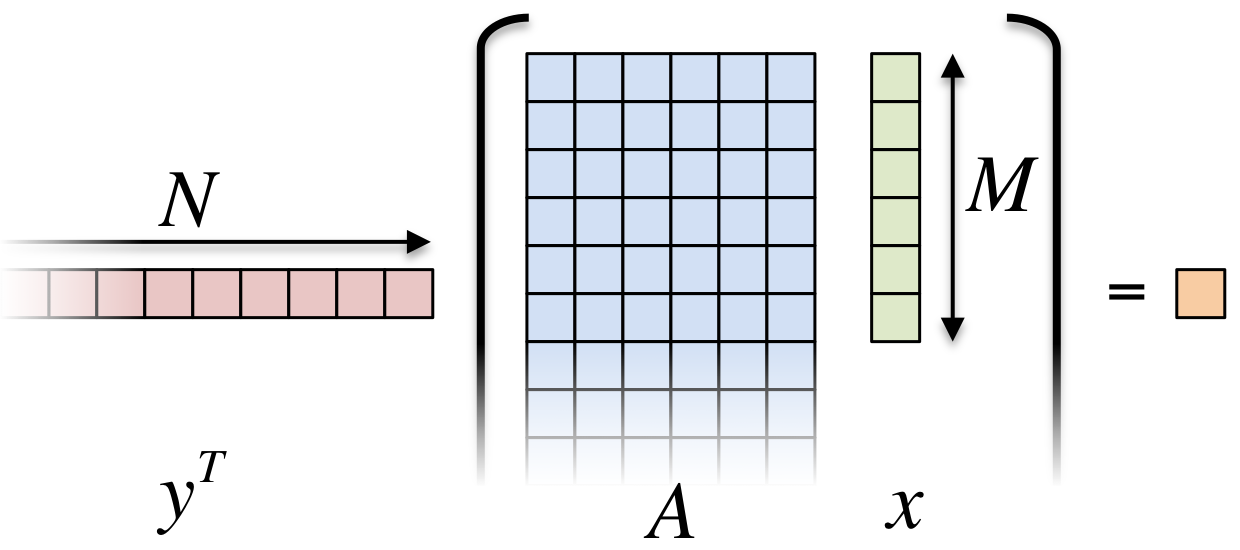
\includegraphics[width=0.8\textwidth]{figures/InnerProductExample_LayoutIntro}
  \end{center}

  \pause
  \vspace{-8pt}

 \textbf{Driving question:} How should {\color{blue}\texttt{A}} be laid out in memory?

  \vspace{8pt}

\end{frame}

%==========================================================================

\begin{frame}[fragile]{Example: inner product (1)}

  Layout is the mapping of multi-index to memory:

  \vspace{-10pt}

  \begin{columns}[t,onlytextwidth]
    \column{.40\textwidth}

      \vspace{20pt}

      \ul{\textbf{LayoutLeft}} \\
      \vspace{3pt}
      \hspace{10pt} in 2D, ``column-major''

      \vspace{50pt}

      \ul{\textbf{LayoutRight}} \\
      \vspace{3pt}
      \hspace{10pt} in 2D, ``row-major''
    \column{.60\textwidth}
      \begin{center}
        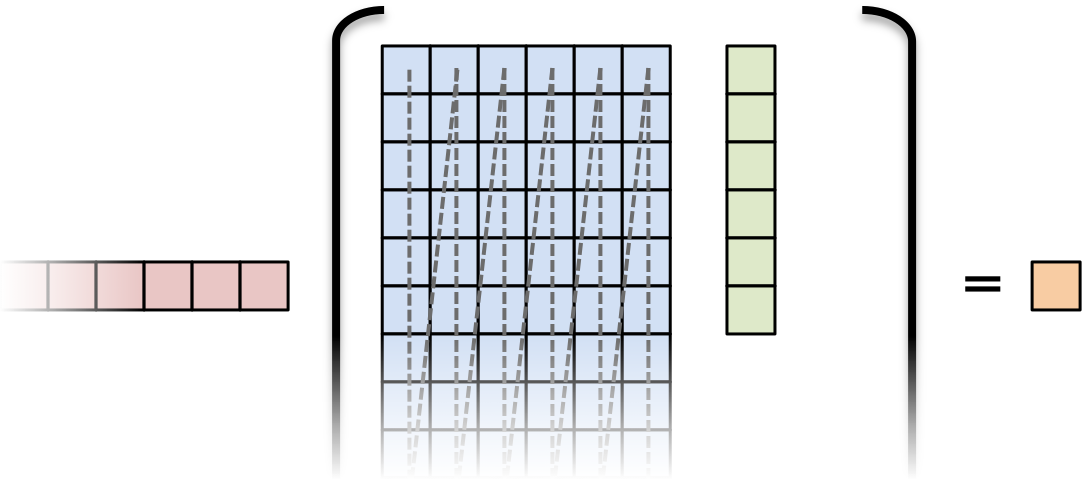
\includegraphics[width=1.00\textwidth]{figures/InnerProductExample_LayoutLeft}
        \\
        \vspace{10pt}
        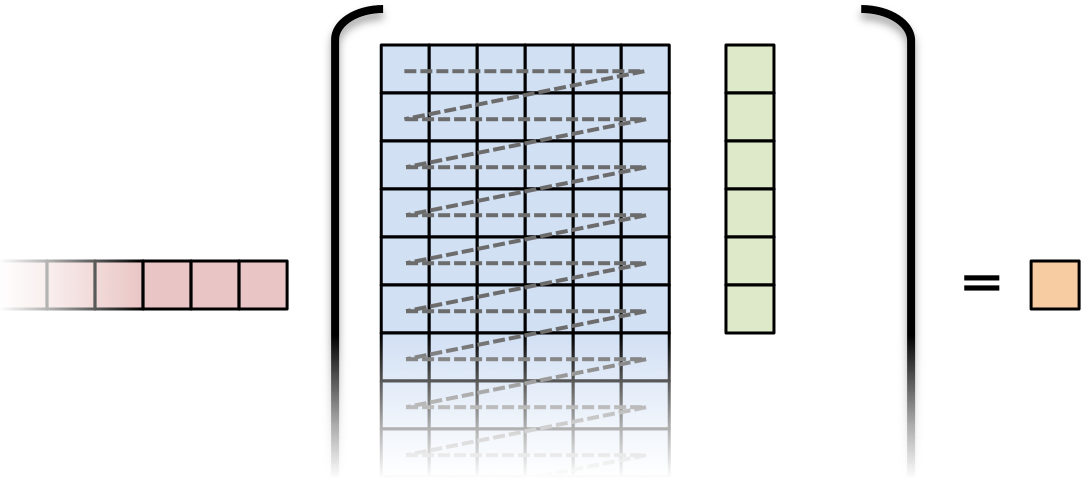
\includegraphics[width=1.00\textwidth]{figures/InnerProductExample_LayoutRight}
      \end{center}
  \end{columns}

\end{frame}

%==========================================================================

\begin{frame}[fragile]{Layout}

  \begin{block}{Important concept: Layout}
    Every \texttt{View} has a multidimensional array \texttt{Layout} set at compile-time.
  \end{block}

  \vspace{5pt}

  \begin{code}[frame=single, keywords={}]
View<double***, @boldLayout@bold, Space> name(...);
  \end{code}

  \pause
  \vspace{-5pt}

  \begin{itemize}
    \item{Most-common layouts are \texttt{LayoutLeft} and \texttt{LayoutRight}. \\
      \hspace{10pt} \texttt{LayoutLeft}: left-most index is stride 1.\\
      \hspace{10pt} \texttt{LayoutRight}: right-most index is stride 1.}
    \item{If no layout specified, default for that memory space is used. \\
      \hspace{10pt} \texttt{LayoutLeft} for \texttt{CudaSpace}, \texttt{LayoutRight} for \texttt{HostSpace}.}
    \item{Layouts are extensible: $\approx$ 50 lines}
    \item{Advanced layouts: \texttt{LayoutStride}, \texttt{LayoutTiled}, ...}
  \end{itemize}

  \vspace{-15pt}

\end{frame}

%==========================================================================

\begin{frame}[fragile]{Exercise \#4: Inner Product, Flat Parallelism}

  \textbf{Details}:
  \begin{small}
  \begin{itemize}
\item Location: \ExerciseDirectory{04/Begin}
\item Replace \texttt{``N''} in parallel dispatch with \texttt{RangePolicy<ExecSpace>}
\item Add \texttt{MemSpace} to all \texttt{Views} and \texttt{Layout} to \texttt{A}
\item Experiment with the combinations of \texttt{ExecSpace}, \texttt{Layout} to view performance
\end{itemize}
  \end{small}


\ul{\textbf{Things to try:}}
  \begin{small}
  \begin{itemize}
  \item Vary problem size and number of rows (-S ...; -N ...)
  \item Change number of repeats (-nrepeat ...)
  \item Compare behavior of CPU vs GPU
  \item On GPUs, compare using \texttt{SharedSpace} vs using the default memory space, i.e, not providing an explicit memory space.
  \item Check what happens if \texttt{MemSpace} and \texttt{ExecSpace} do not match.
  \end{itemize}
  \end{small}
\end{frame}

%==========================================================================

\begin{frame}[fragile]{Exercise \#4: Inner Product, Flat Parallelism}


  \vspace{-5pt}
  \hspace{-15pt}
    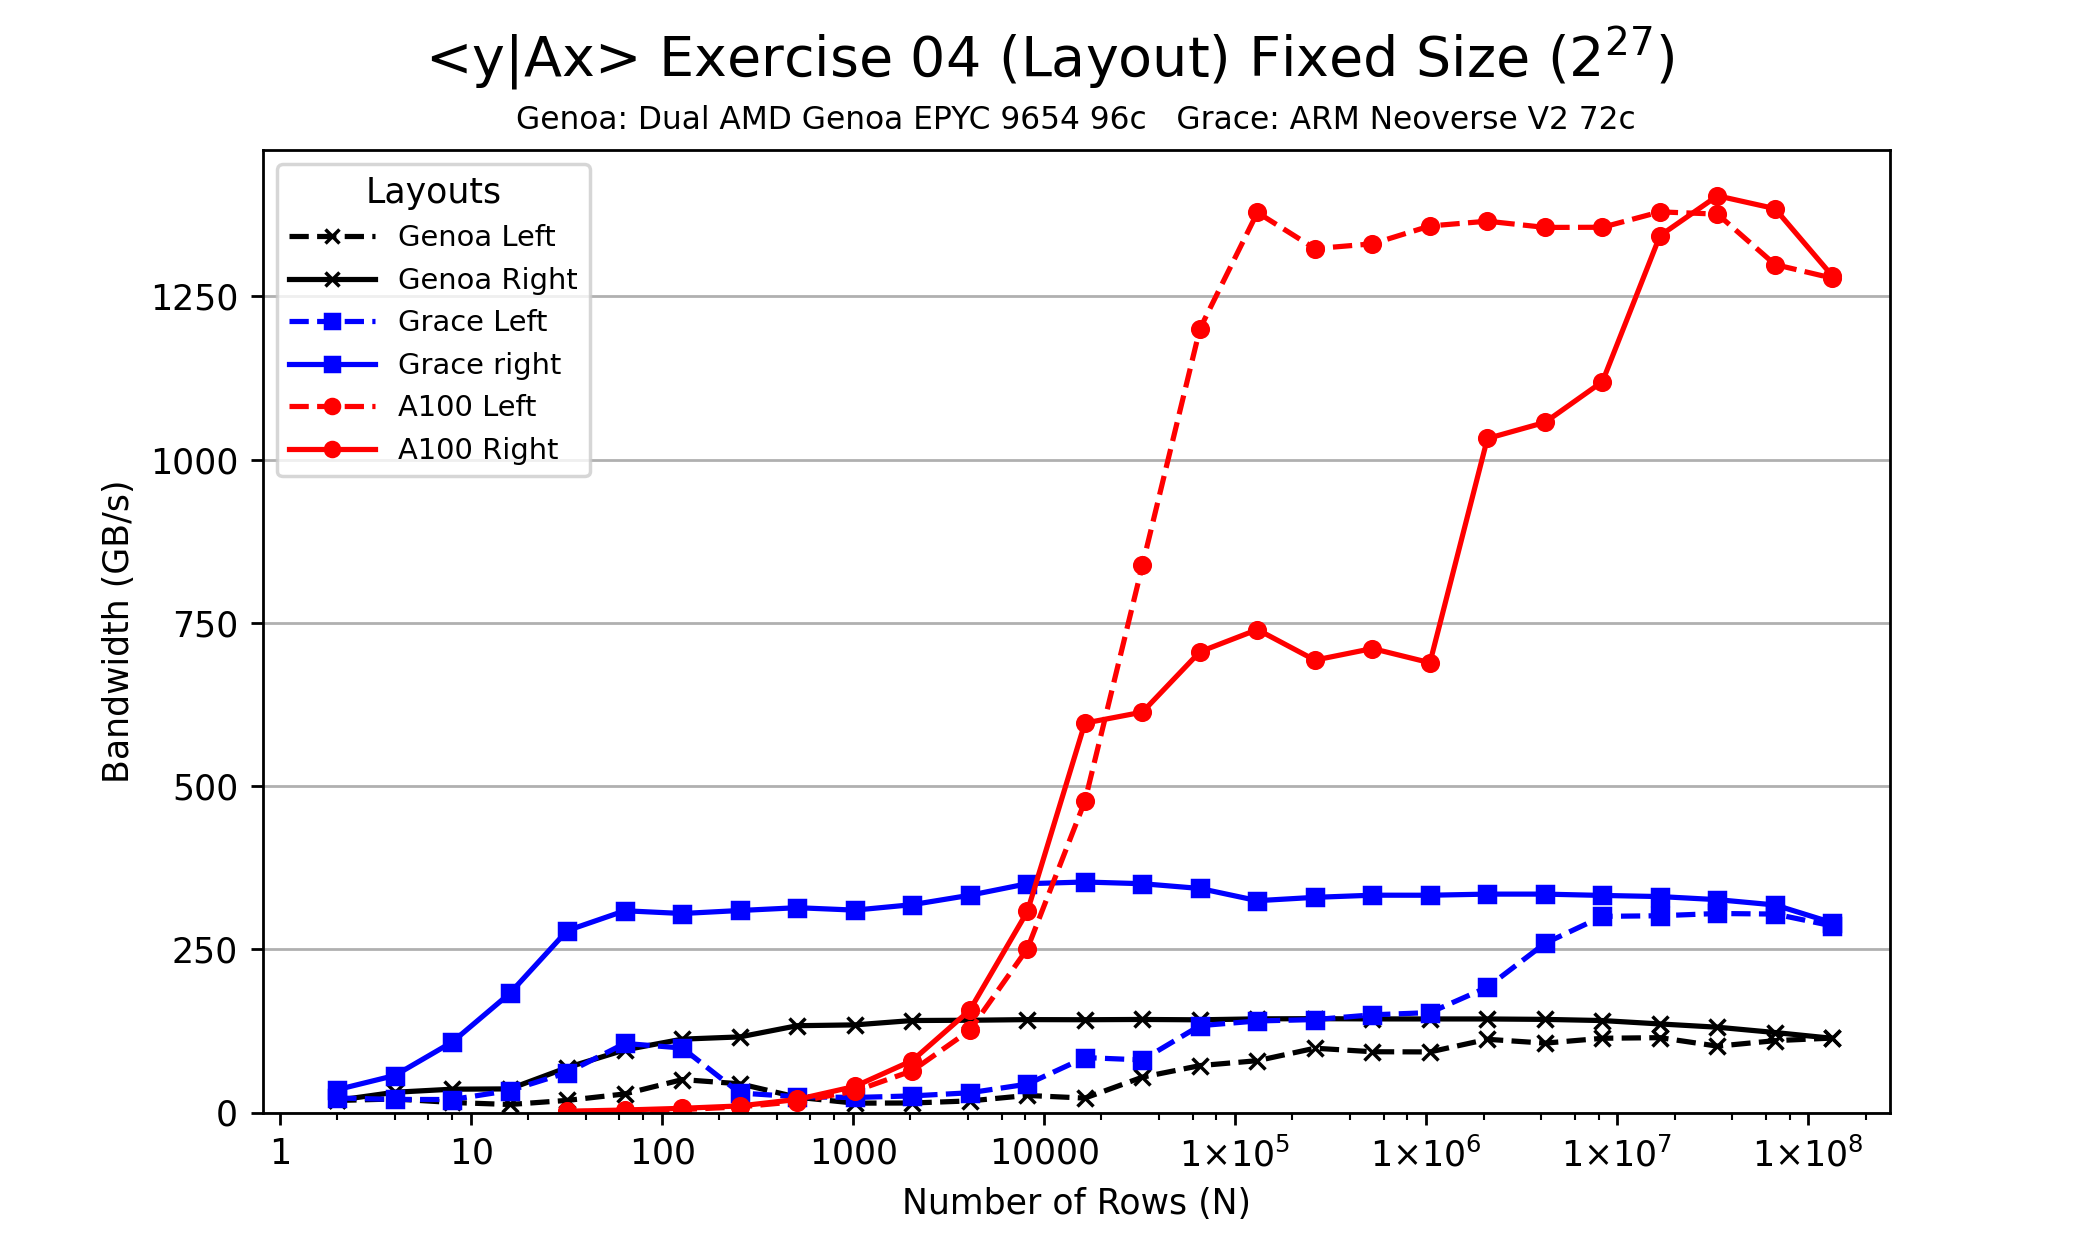
\includegraphics[trim=20pt 0 50pt 5pt, clip, width=1.0\textwidth]{figures/Exercise04-Performance.png}
  \vspace{-15pt}

  \begin{textblock*}{0.5\textwidth}(0.97\textwidth,0.50\textheight)
    \textbf{\LARGE Why?}
  \end{textblock*}

\end{frame}

%==========================================================================

\begin{frame}[fragile]{Caching and coalescing (0)}

  \ul{\textbf{Thread independence:}}

  \begin{code}[keywords={}]
operator()(int index, double & valueToUpdate) const {
  const double d = _data(index);
  valueToUpdate += d;
}
  \end{code}

  Question: once a thread reads \texttt{d}, does it need to wait?

  \pause

  \begin{itemize}
    \item \textbf{CPU} threads are independent.
       \begin{itemize}
	   \item i.e., threads may execute at any rate.
       \end{itemize}
  \item<3->{\textbf{GPU} threads execute synchronized. 
	  \begin{itemize}
	     \item i.e., threads in groups can/must execute instructions together.
	  \end{itemize}}
  \end{itemize}

  \pause
  \pause

	In particular, all threads in a group (\emph{warp} or \emph{wavefront}) must finished their loads before \emph{any} thread can move on.

  \vspace{5pt}

  \pause

  So, \textbf{how many cache lines} must be fetched before threads can move on?

\end{frame}

%==========================================================================

\ifmedium
\begin{frame}[fragile]{Caching and coalescing (1)}

  \ul{\textbf{CPUs}: few (independent) cores with separate caches:}

  \vspace{-10pt}

  \begin{columns}[t,onlytextwidth]
    \column{.50\textwidth}
      \begin{center}
        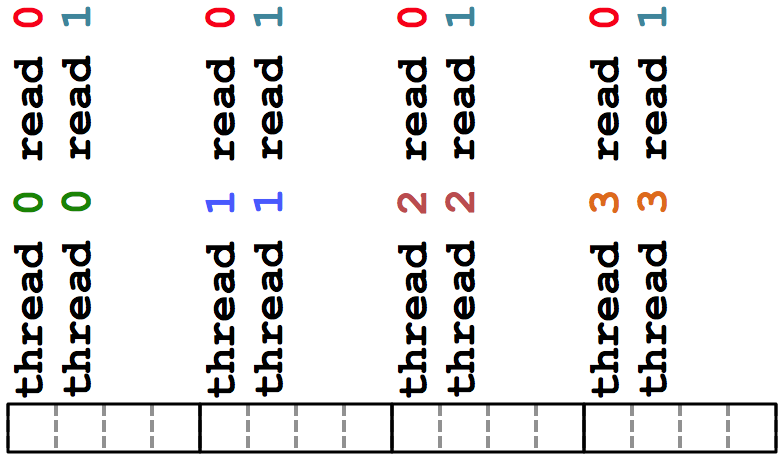
\includegraphics[width=0.80\textwidth]{figures/MemoryAccessPatterns_Caching}
      \end{center}
    \column{.50\textwidth}
      \begin{center}
        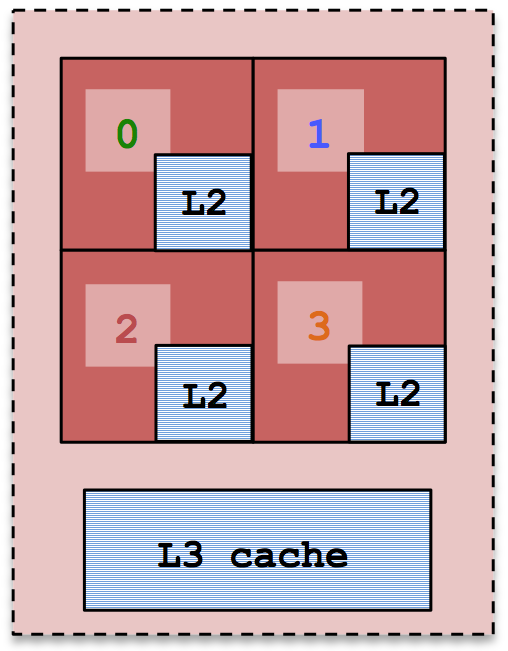
\includegraphics[width=0.38\textwidth]{figures/Schematics_CPU_withThreadIndices_justOne}
      \end{center}
  \end{columns}

  \vspace{5pt}
  \pause

  \ul{\textbf{GPUs}: many (synchronized) cores with a shared cache:}

  \vspace{-10pt}

  \begin{columns}[t,onlytextwidth]
    \column{.50\textwidth}
      \begin{center}
        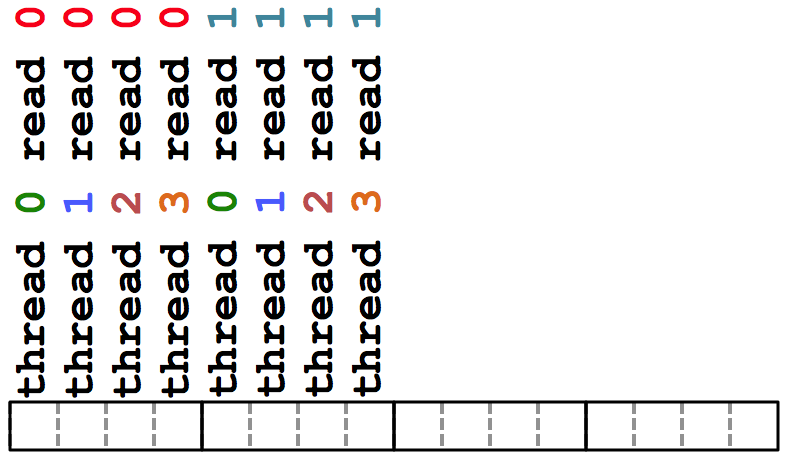
\includegraphics[width=0.80\textwidth]{figures/MemoryAccessPatterns_Coalescing}
      \end{center}
    \column{.50\textwidth}
      \begin{center}
        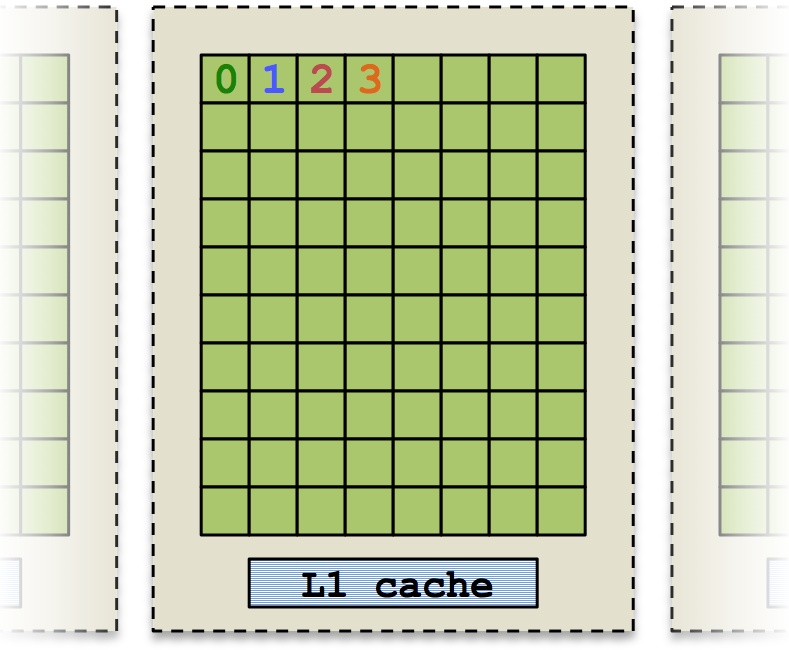
\includegraphics[width=0.60\textwidth]{figures/Schematics_GPU_withThreadIndices}
      \end{center}
  \end{columns}

\end{frame}
\fi

%==========================================================================

\begin{frame}[fragile]{Caching and coalescing (2)}

  \begin{block}{Important point}
    For performance, accesses to views in \texttt{HostSpace} must be \textbf{cached}, while access to views in \texttt{CudaSpace} must be \textbf{coalesced}.
  \end{block}

  \vspace{5pt}

  \textbf{Caching}: if thread \texttt{t}'s current access is at position \texttt{i}, \\
  \hspace{20pt} thread \texttt{t}'s next access should be at position \texttt{i+1}.

  \vspace{5pt}

  \textbf{Coalescing}: if thread \texttt{t'}s current access is at position \texttt{i}, \\
  \hspace{20pt} thread \texttt{t+1}'s current access should be at position \texttt{i+1}.

  \pause

  \begin{alertblock}{Warning}
    Uncoalesced access on GPUs and non-cached loads on CPUs \emph{greatly} reduces performance (can be 10X)
  \end{alertblock}

\end{frame}

%==========================================================================

\ifmedium
\begin{frame}[fragile]{Mapping indices to cores (0)}

  Consider the array summation example:

  \begin{code}[keywords={}]
View<double*, @boldSpace@bold> data("data", size);
...populate data...

double sum = 0;
Kokkos::parallel_reduce("Label", 
  RangePolicy< @boldSpace@bold>(0, size),
  KOKKOS_LAMBDA (const size_t index, double & valueToUpdate) {
    valueToUpdate += data(index);
  },
  sum);
  \end{code}

  \vspace{0pt}

  Question: is this cached (for \texttt{OpenMP}) and coalesced (for \texttt{Cuda})?

  \pause
  \vspace{5pt}

  Given \texttt{P} threads, \textbf{which indices} do we want thread 0 to handle?

  \vspace{-15pt}

  \begin{columns}[t,onlytextwidth]
    \column{.50\textwidth}
      \begin{center}
        Contiguous: \\
        \texttt{0, 1, 2, ..., N/P}
      \end{center}
    \column{.50\textwidth}
      \begin{center}
        Strided: \\
        \texttt{0, N/P, 2*N/P, ...}
      \end{center}
  \end{columns}

  \vspace{-10pt}
  \pause

  \begin{columns}[t,onlytextwidth]
    \column{.50\textwidth}
      \begin{center}
        \textbf{CPU}
      \end{center}
    \column{.50\textwidth}
      \begin{center}
        \textbf{GPU}
      \end{center}
  \end{columns}

  \vspace{-10pt}

  \begin{center}
    \textbf{Why?}
  \end{center}

  \vspace{-10pt}

\end{frame}
\fi

%==========================================================================

\ifmedium
\begin{frame}[fragile]{Mapping indices to cores (1)}

  \ul{\textbf{Iterating for the execution space:}}

  \begin{code}[keywords={}]
operator()(int index, double & valueToUpdate) const {
  const double d = _data(index);
  valueToUpdate += d;
}
  \end{code}

  \vspace{5pt}

  As users we don't control how indices are mapped to threads, so how do we achieve good memory access?

  \pause
  \vspace{3pt}

  \begin{block}{Important point}
    Kokkos maps indices to cores in \textbf{contiguous chunks} on CPU execution spaces, and \textbf{strided} for \texttt{Cuda}.
  \end{block}

\end{frame}
\fi

%==========================================================================

\begin{frame}[fragile]{Mapping indices to cores (2)}

  \begin{block}{Rule of Thumb}
    Kokkos index mapping and default layouts provide efficient access if \textbf{iteration indices} correspond to the \textbf{first index} of array.
  \end{block}

  \vspace{10pt}

  \textbf{Example:}

  \vspace{5pt}

  \begin{code}[keywords={}, frame=single]
  View<double***, ...> view(...);
  ...
  Kokkos::parallel_for("Label", ... ,
    KOKKOS_LAMBDA (int workIndex) {
      ...
      @darkredview(..., ... , workIndex ) = ...@darkred;
      @darkredview(... , workIndex, ... ) = ...@darkred;
      @darkgreenview(workIndex, ... , ... ) = ...@darkgreen;
    });
  ...
  \end{code}

\end{frame}

%==========================================================================

\iffull
\begin{frame}[fragile]{Example: inner product (2)}

  \begin{block}{Important point}
    Performant memory access is achieved by Kokkos mapping parallel work indices \textbf{and} multidimensional array layout \emph{appropriately for the architecture}.
  \end{block}

  \pause
  \vspace{3pt}

  \ul{\textbf{Analysis: row-major} (\texttt{LayoutRight})}

  \vspace{-10pt}

  \begin{center}
    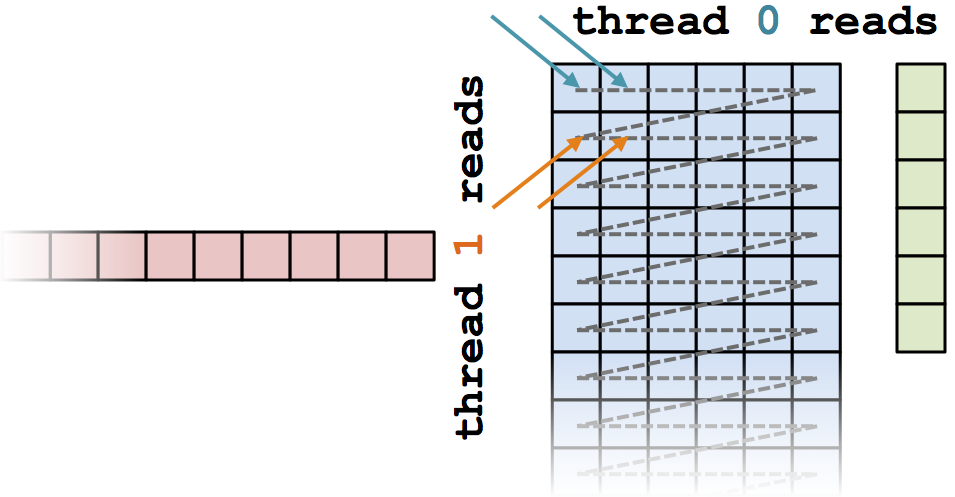
\includegraphics[width=0.65\textwidth]{figures/InnerProductExample_LayoutRight_withThreadReads}
  \end{center}

  \vspace{-28pt}
  \pause

  \begin{itemize}
    \item{\textbf{HostSpace}: cached ({\color{darkgreen}good})}
    \item{\textbf{CudaSpace}: uncoalesced ({\color{red}bad})}
  \end{itemize}

\end{frame}
\fi
\setcounter{subfigure}{0}% Reset subfigure counter


%==========================================================================

\ifmedium
\begin{frame}[fragile]{Example: inner product (3)}

  \begin{block}{Important point}
    Performant memory access is achieved by Kokkos mapping parallel work indices \textbf{and} multidimensional array layout \emph{optimally for the architecture}.
  \end{block}

  \vspace{3pt}

  \ul{\textbf{Analysis: column-major} (\texttt{LayoutLeft})}

  \vspace{-10pt}

  \begin{center}
    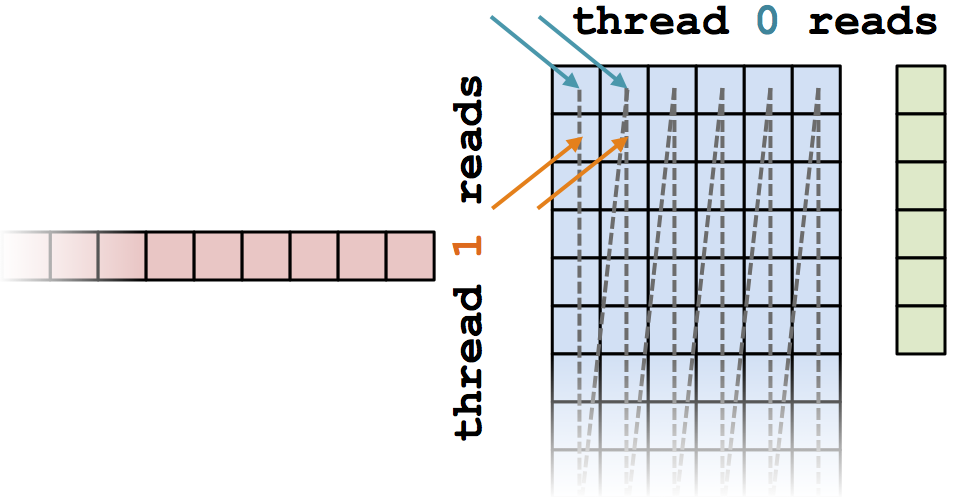
\includegraphics[width=0.65\textwidth]{figures/InnerProductExample_LayoutLeft_withThreadReads}
  \end{center}

  \vspace{-28pt}
  \pause

  \begin{itemize}
    \item{\textbf{HostSpace}: uncached ({\color{red}bad})}
    \item{\textbf{CudaSpace}: coalesced ({\color{darkgreen}good})}
  \end{itemize}

\end{frame}
\fi
\setcounter{subfigure}{0}% Reset subfigure counter

%==========================================================================

\begin{frame}[fragile]{Example: inner product (4)}

  \ul{\textbf{Analysis: Kokkos architecture-dependent}}

  \vspace{-3pt}

  \begin{code}[keywords={}]
View<double**, @boldExecutionSpace@bold> @blueA@blue(N, M);
parallel_for(RangePolicy< @boldExecutionSpace@bold>(0, N),
  ... thisRowsSum += @blueA@blue(j, i) * @darkgreenx@darkgreen(i);
  \end{code}

  \vspace{-20pt}

  \begin{figure}
    \centering
    \subfloat[\texttt{OpenMP}]{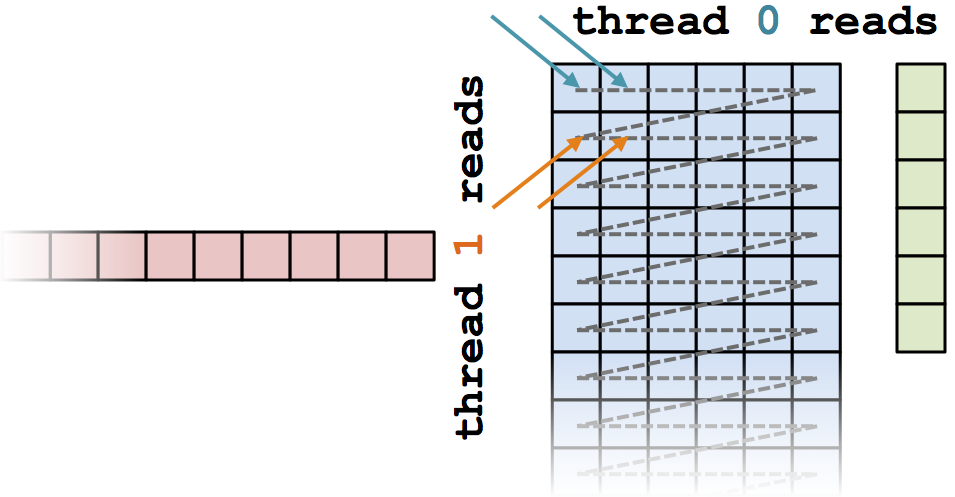
\includegraphics[trim=450pt 0pt 0pt 0pt, clip,width=0.30\textwidth]{figures/InnerProductExample_LayoutRight_withThreadReads}} \qquad
    \subfloat[\texttt{Cuda}]{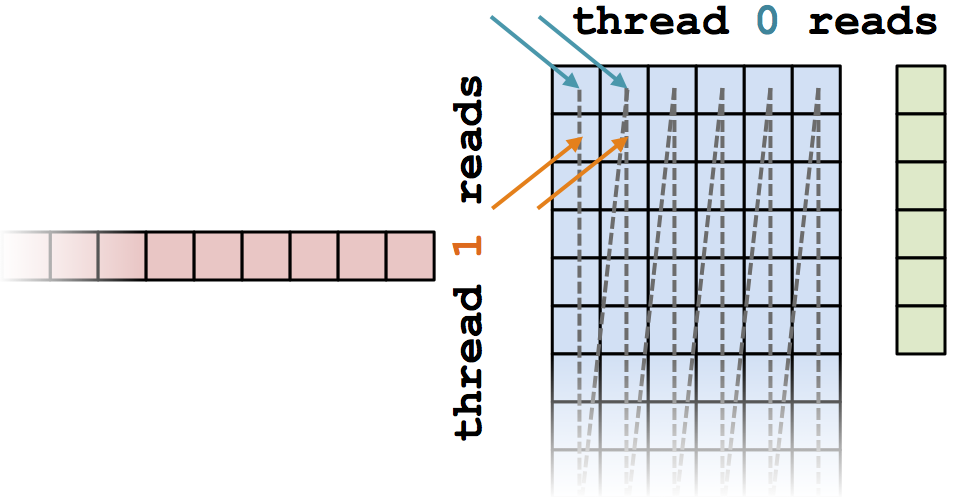
\includegraphics[trim=450pt 0pt 0pt 0pt, clip,width=0.30\textwidth]{figures/InnerProductExample_LayoutLeft_withThreadReads}}
  \end{figure}

  \vspace{-10pt}

  \begin{itemize}
    \item{\textbf{HostSpace}: cached ({\color{darkgreen}good})}
    \item{\textbf{CudaSpace}: coalesced ({\color{darkgreen}good})}
  \end{itemize}

\end{frame}
\setcounter{subfigure}{0}% Reset subfigure counter

%==========================================================================

\begin{frame}[fragile]{Example: inner product (5)}

  \vspace{-5pt}
  \hspace{-15pt}
    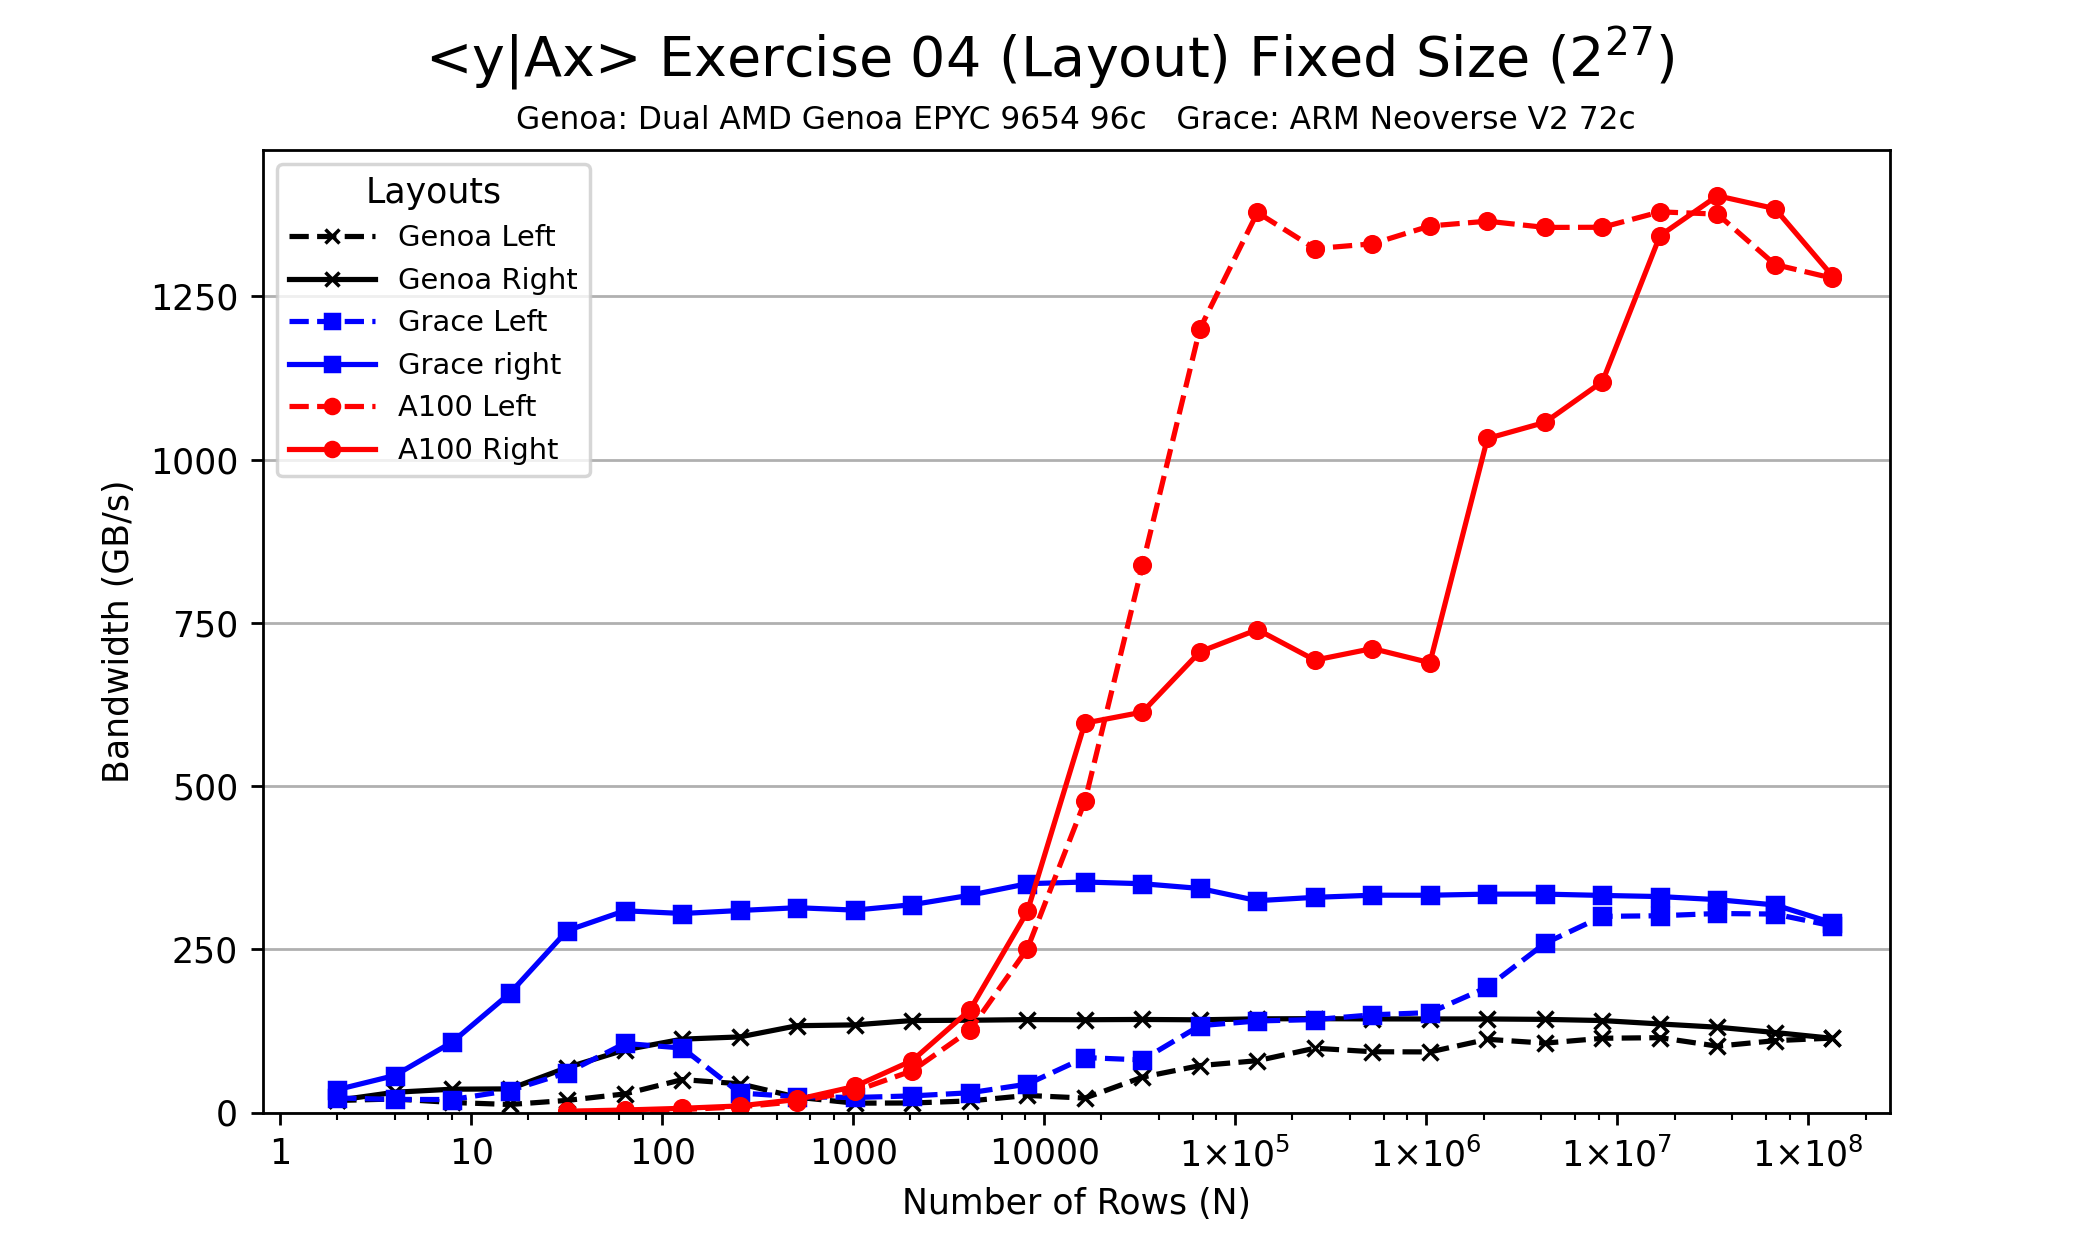
\includegraphics[trim=20pt 0 50pt 5pt, clip, width=1.0\textwidth]{figures/Exercise04-Performance.png}
  \vspace{-15pt}

  \begin{textblock*}{0.5\textwidth}(0.69\textwidth,0.30\textheight)
    \textbf{coalesced}
  \end{textblock*}

  \begin{textblock*}{0.5\textwidth}(0.35\textwidth,0.65\textheight)
    \textbf{cached}
  \end{textblock*}

  \begin{textblock*}{0.5\textwidth}(0.65\textwidth,0.56\textheight)
    \textbf{uncoalesced}
  \end{textblock*}

  \begin{textblock*}{0.5\textwidth}(0.71\textwidth,0.78\textheight)
    \textbf{uncached}
  \end{textblock*}

\end{frame}

%==========================================================================

\begin{frame}{Memory Access Pattern Summary}

  \begin{itemize}
    \item{Every \texttt{View} has a \texttt{Layout} set at compile-time through a \textbf{template parameter}.}
    \item{\texttt{LayoutRight} and \texttt{LayoutLeft} are \textbf{most common}.}
    \item{\texttt{Views} in \texttt{HostSpace} default to \texttt{LayoutRight} and \texttt{Views} in \texttt{CudaSpace} default to \texttt{LayoutLeft}.}
    \item{Layouts are \textbf{extensible} and \textbf{flexible}.}
    %\item{Correct memory access pattern is \textbf{essential} for performance.}
    \item{For performance, memory access patterns must result in \textbf{caching} on a CPU and \textbf{coalescing} on a GPU.}
    \item{Kokkos maps parallel work indices \textit{and} multidimensional array layout for \textbf{performance portable memory access patterns}.}
    \item{There is \textbf{nothing in} \texttt{OpenMP}, \texttt{OpenACC}, or \texttt{OpenCL} to manage layouts.}\\
    $\Rightarrow$ You'll need multiple versions of code or pay the performance penalty.
  \end{itemize}

\end{frame}
